% !TeX spellcheck = ru_RU
%pdflatex, utf8
\documentclass[unicode, 10pt, a5paper, oneside]{article}

% Установка полей страницы
%\usepackage{anysize}
%\marginsize{0.3cm}{0.3cm}{0.3cm}{0.3cm}
\usepackage[a5paper, margin=0.3cm, bindingoffset=0cm]{geometry}

% Поддержка русского языка
\usepackage[T2A]{fontenc}		% Корректная кодировка шрифта при использовании cm-super
\usepackage[utf8]{inputenc}		% Кодировка ввода
\usepackage[russian]{babel}		% Словарь расстановки переносов
%\usepackage{cmap}				% Перекодировка символов в pdf при использовании обычного cm

% Всякие математические фишки
\usepackage{amsmath}
\usepackage{amsfonts}
\usepackage{amssymb}

% Изменение цвета, работа с графикой
\usepackage{color}
\usepackage[pdftex]{graphicx}
\graphicspath{{images/}}

% Команда для вставки ссылок \url{URL}
\usepackage[hyphens]{url}
\urlstyle{rm}					% Стиль шрифта ссылок: с засечками

% Кликабельные ссылки внутри документа
\usepackage[unicode]{hyperref}

% Включает отступ у первого абзаца в разделе
\usepackage{indentfirst}

% Настрйока стиля списков
\usepackage{enumitem}
\setlist{noitemsep, leftmargin=*, labelindent=\parindent, topsep=0pt, parsep=0pt, partopsep=0pt}

\setlist[itemize,1]{label=$\diamond$}
\setlist[itemize,2]{label=\textendash}
\setlist[itemize,3]{label=$\star$}

\renewcommand{\alph}[1]{\asbuk{#1}} % Костыль для кирилической нумерации вместо латинской
\setlist[enumerate,1]{label=\arabic*)}
\setlist[enumerate,2]{label=\alph*)}
\setlist[enumerate,3]{label=(\arabic*)}


\usepackage{textcomp}			% Команды для вставки разных символов (градусы, проценты, итд)
\usepackage{float}				% Размещение плавающих объектов там где они созданы (X)
\usepackage{wrapfig}			% Обтекаемые текстом рисунки

% Подписи у флоатов
\setlength{\intextsep}{0pt} % Отстут вокруг плавающих окружений
\usepackage{caption}
\captionsetup{parskip=0pt}
\captionsetup[figure]{labelsep=period,justification=centering,singlelinecheck=false,textfont=small,labelfont=small,aboveskip=2pt,belowskip=0pt}

% Изменение формата заголовков разделов
\usepackage{titlesec}
\titleformat{\section}{\newpage\small\bfseries}{\thesection. }{0pt}{}{}
\titlespacing*{\section}{0pt}{0pt}{0pt}

\titleformat{\subsection}{\small\bfseries}{\thesubsection. }{0pt}{}{}
\titlespacing*{\subsection}{0pt}{0pt}{0pt}

\usepackage{array}				% Позволяет объявить свои типы колонок
\usepackage{calc}				% Математика, исп-ся для расчёта ширины колонки
\usepackage{longtable}			% Длинные таблицы

% Минимальный отступ в таблицах
\setlength{\tabcolsep}{1.5mm}

% Новые типы колонок. Ширина задётся как доля от linewidth
\newcolumntype{L}[1]{p{#1\linewidth-2\tabcolsep-2\arrayrulewidth}}
\newcolumntype{C}[1]{>{\centering}p{#1\linewidth-2\tabcolsep-2\arrayrulewidth}}
\newcolumntype{R}[1]{>{\raggedleft}p{#1\linewidth-2\tabcolsep-2\arrayrulewidth}}
\newcolumntype{U}[2]{p{#1\linewidth-(#2)}}

% Стараться не оставлять одиноких строк в начале и конце абзаца
\clubpenalty=1000
\widowpenalty=1000

% Расстановка отступов и переносов
\emergencystretch=2.5em			% Максимальный промежуток между словами
\tolerance=2000
\frenchspacing


\begin{document}

\setcounter{section}{30}

% Вопрос 31 ---------------------------------------------------------------------------------------------------------------
\section{Показатели качества ЭС.}

Показатели качества продукции --- количественная характеристика определенного свойства продукции на определенном этапе жизненного цикла.

Показатели качества продукции делятся на следующие группы:
\begin{enumerate}
\item Назначения
\item Надежности
\item Технологичности
\item Эргономические
\item Эстетические
\item Стандартизация и унификация
\item Патентно-правовые
\item Экономические
\end{enumerate}

Единичный показатель качества --- показатель качества продукции, относящийся только к одному из её свойств. Комплексный показатель качества --- показатель качества продукции, относящийся к нескольким её свойствам.

% Вопрос 32 ---------------------------------------------------------------------------------------------------------------
\section{Управление качеством ЭС.}

Управление качеством продукции базируется на статических методах контроля, зародилось в 30-е годы в связи с переходом к массовому производству изделий. В связи с этим стали применять выборочный контроль продукции с оценкой его результатов статистическим методом.
Контроль качества базируется на статистических методах и развиваясь циклически проходит через определенные этапы (см. рис)
\begin{center}
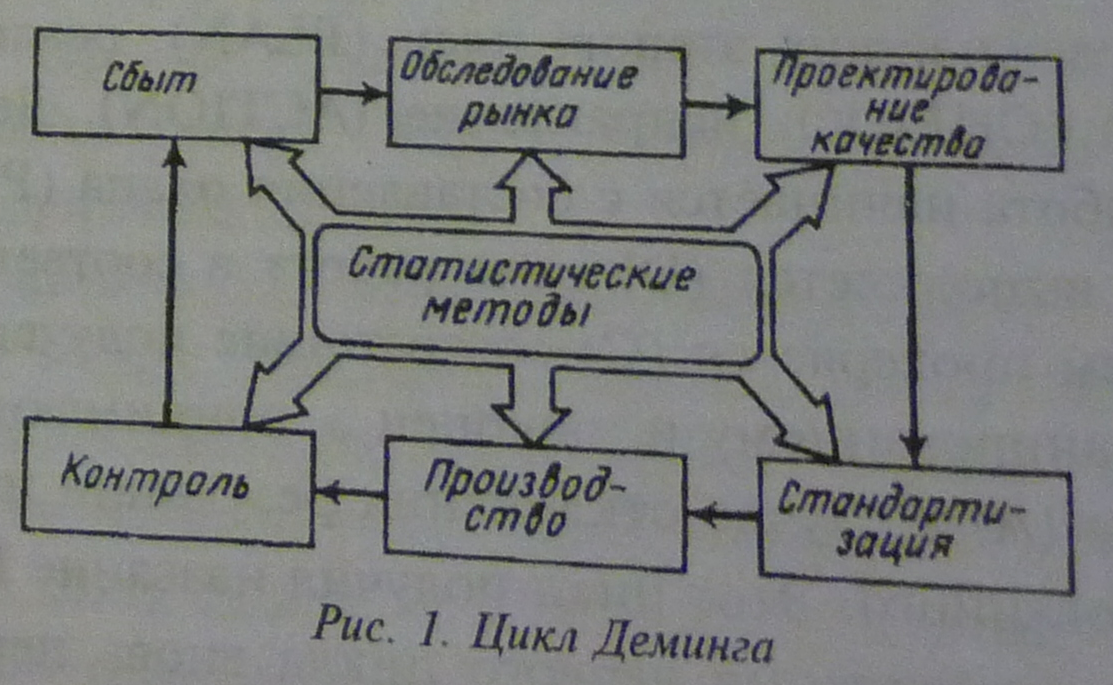
\includegraphics[width=0.6\textwidth]{32_Demming.png}
\end{center}

Управление качеством продукции базируется на статических методах контроля, зародилось в 30-е годы в связи с переходом к массовому производству изделий. В связи с этим стали применять выборочный контроль продукции с оценкой его результатов статистическим методом.

Контроль качества базируется на статистических методах и развиваясь циклически проходит через определенные этапы

Для эффективного обеспечения контроля качества необходимо участие всех, без исключения, работников предприятия. Такой контроль качества называется Тотальным(TQC). Был придуман и внедрен впервые в Японии 60х годах.

Среди статистических методов можно выделить 7 наиболее эффективных  и доступных:
\begin{enumerate}
\item	Расслоение графики (полигон, гистограмма, кумулятивная кривая)
\item	Расслоение общей изменчивости статистических данных с помощью дисперсионного анализа.
\item	Диаграмма Парето
\item	Причинно-следственная диаграмма
\item	Диаграмма разброса (поле корреляции)
\item	Контрольная карта
\item	Контрольный лист
\end{enumerate}


% Вопрос 33 ---------------------------------------------------------------------------------------------------------------
\section{Себестоимость и уровень качества ЭС.}

Зависимость себестоимости и уровня качества продукции можно в общем виде представить в виде следующего графика (рис.)

СП --- затраты на материалы, комплектующие  изделия, оборудование, заработную плату, контроль и испытания и т.д.

\begin{figure}[H]
\centering 
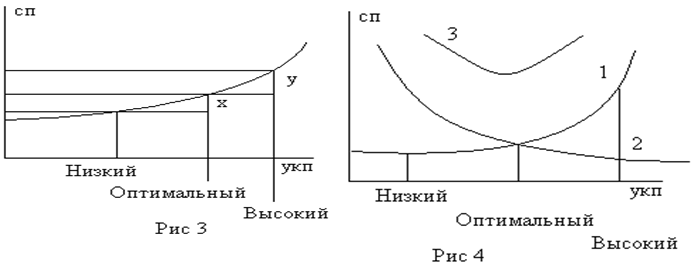
\includegraphics[width=0.7\textwidth]{33_Sebestoim.png}
\caption{Слева -- зависимость себестоимости от уровня качества, справа --оптимальный уровень качества при затратах на изготовление и эксплуатацию.}
\end{figure}

При повышении уровня качества от низкого до оптимального затраты растут медленно (х), поскольку производство легко справляется с заданными требованиями на уровень качества. По мере повышения УКП затраты (у) существенно возрастают. При дальнейшем повышении требований к УКП в конце концов достигается такой предел, когда ни оборудование, ни ТП, ни НТП и т.д. не в состоянии обеспечить требуемого (недостижимо высокого) качества. Затраты при этом устремляются в бесконечность.

Затраты на продукцию складываются из затрат на изготовление (проектирование и производство) и на эксплуатацию продукции (рис.).

Оптимальный уровень качества продукции --- это такой уровень, выше или ниже которого производить продукцию экономически нецелесообразно.
При низком уровне качества продукции в сфере эксплуатации потребитель вынужден выделять дополнительные средства на ремонт, доработку и обслуживание продукции.
Высокий уровень качества продукции обуславливается ее высокой себестоимостью. 


\begin{enumerate}
\item Расслоение графики (полигон, гистограмма, кумулятивная кривая)
\item Расслоение общей изменчивости статистических данных с помощью дисперсионного анализа.
\item Диаграмма Парето
\item Причинно-следственная диаграмма
\item Диаграмма разброса (поле корреляции)
\item Контрольная карта
\item Контрольный лист
\end{enumerate}


% Вопрос 34 ---------------------------------------------------------------------------------------------------------------
\section{Корреляционная связь показателей ЭС.}

Диаграмма разброса применяется для исследования зависимости (корреляции) между двумя видами данных. Поэтому её часто называют полем корреляции.
С помощью диаграммы разброса удобно наблюдать процесс изменения параметра качества во времени при воздействии тех или иных факторов.

Совокупность точек на графике --- диаграмма рассеяния.
С помощью диаграммы разброса можно определить имеется ли связь между параметрами и вид корреляции.(прямая корреляция, легкая прямая корреляция, обратная корреляция, легкая обратная корреляция, отсутствие корреляции, криволинейная корреляция.)

\begin{figure}[H]
\centering 
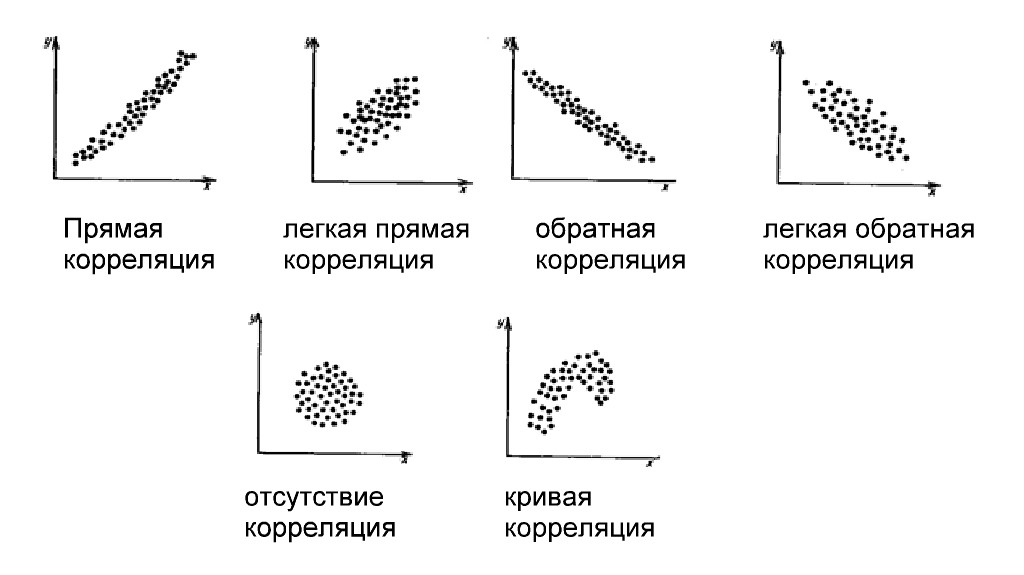
\includegraphics[width=0.8\textwidth]{34_Korelyacia2.JPG}
\caption{Виды корреляции}
\end{figure}

Криволинейную корреляцию можно разделить на участки, имеющие прямолинейный характер, и исследовать каждый участок в отдельности.

Степень связи может быть оценена: коэффициентом корреляции (прямолинейная), корреляционным отношением (криволинейная).

Связь прямолинейную между Х и У можно найти:
\begin{equation}
Y-m_Y = r \cdot \frac{S_X}{S_Y} \cdot (X-m_Y),
\end{equation}
где r --- коэффициент парной корреляции,
\begin{equation}
r = \frac{\sum_{i=1}^n (X_i - m_X)(Y_i-m_Y)}{(n-1) \cdot S_X \cdot S_Y},
\end{equation} 
\begin{equation}
m_X = \dfrac{\sum_{i=1}^n X_i}{n}; S_X=\sqrt{\dfrac{\sum_{i=1}^n (X_i -m_X)^2}{n-1}},
\end{equation}

n --- число пар наблюдений.

$ -1 \leqslant r \leqslant 1$

При |r|=1 --- связь функциональная (зависимость между параметрами ввиде формул),

при |r|<1 --- связь статическая. Каждому фиксированному значению Х соответствует ряд изменяющихся вместе с Х значений У и наоборот. Параметры Х и У считаются статистически зависимыми, если
\begin{center} 
$\dfrac{\mid r \mid \cdot \sqrt{n-2}}{\sqrt{1-r^{2}}} \geqslant t_T = f(\alpha ; \nu = n-2)$\\
\end{center}

Знак говорит о связи значений, если «-» то при уменьшении значения Х , У увеличивается и наоборот. Если «+» то при увеличении Х увеличивается и У.
При r = 0 Х и У не связаны  между собой и не зависят друг от друга.


% Вопрос 35 ---------------------------------------------------------------------------------------------------------------
\section{Метод расслаивания <<4М>>.}

Простой и эффективный статистический метод, широко используемый в системе УК, --- метод расслаивания

В основе метода --- расслаивание статистических данных (т.е. группировка данных) в зависимости от условия их получения и обработка каждой группы в отдельности. Данные, разделённые на группы в соответствии с их особенностями, называют слоями (стратами), а сам процесс разделения на слои --- расслаиванием (стратификацией). Существуют различные методы расслаивания, применение которых зависит от конечных задач. В производственных условиях обычно используется метод 4М, учитывающий факторы, зависящие от человека, машины, материала, метода. Расслаивание осуществляется:
\begin{enumerate}
\item по исполнителям --- квалификации, полу, стажу работы и т.п.;
\item по оборудованию --- году выпуска, марке, типу конструкции  и т.п.;
\item по материалу --- месту производства, фирме-производителю и т.п.;
\item по способу производства 

\end{enumerate}

В результате расслаивания обязательно должны соблюдаться два условия:
\begin{itemize}
\item различия между значениями СВ внутри слоя должны быть как можно меньше по сравнению с различием её значений в не расслоенной исходной совокупности;
\item различие между слоями  должно быть как можно больше.
\end{itemize}	

При контроле качества изготовления изделий на практике возникает задача предполагаемого источника ухудшения качества продукции, когда разброс значений параметра качества около среднего значения возрастает. В случае нормального закона распределения контролируемого параметра качества такую информацию возможно получить путём расслаивания дисперсии с помощью дисперсионного анализа.

% Вопрос 36 ---------------------------------------------------------------------------------------------------------------
\section{Метод <<АВС-анализ>>.}

Метод служит для эффективности контроля качества изделия, для этого все изделия разбиваются по ценовым диапазонам (или иным критериям), составляется таблица,\\
\begin{center}
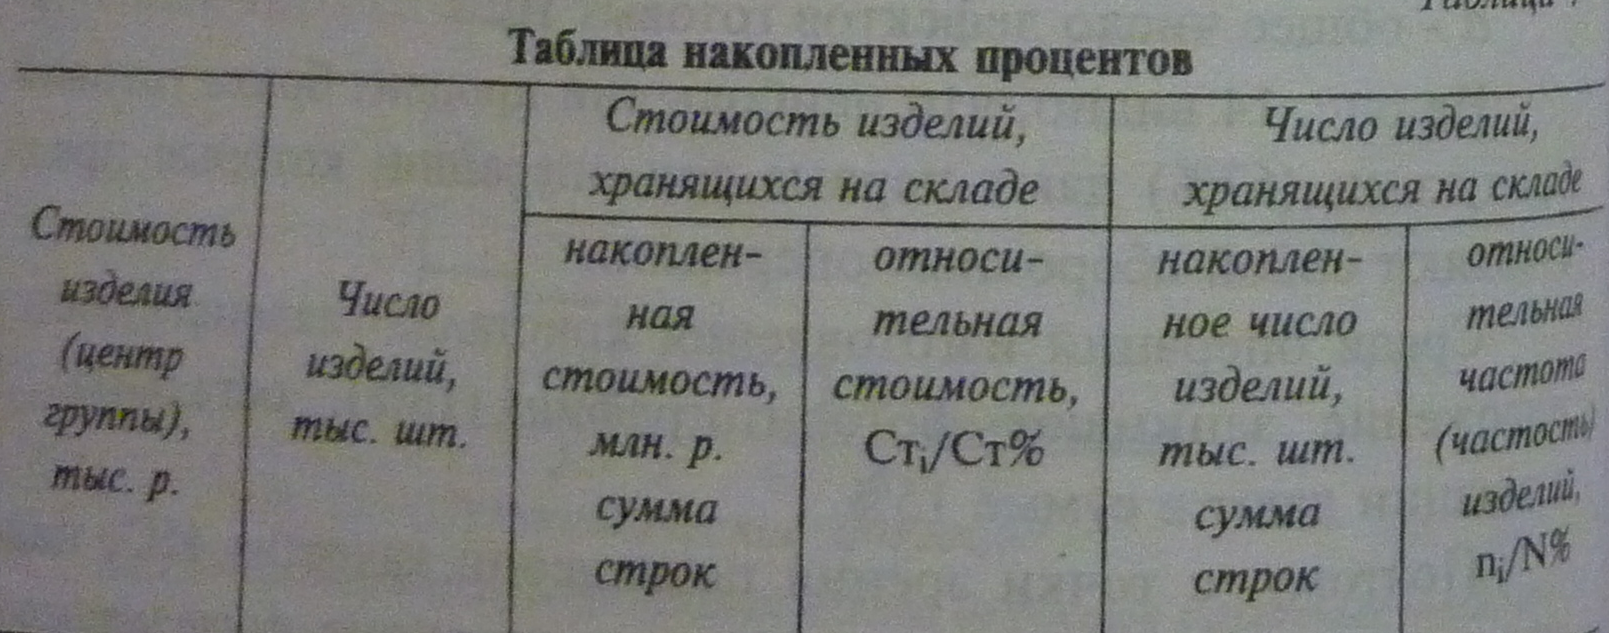
\includegraphics[width=0.7\textwidth]{36_Shapka.png}
\end{center}
и строится диаграмма Парето (по оси У откладывается относительная стоимость изделия в \%, а по оси Х относительная частость изделий в\%). По результатам которой можно выделить три группы: группа А --- наиболее дорогие изделия и её контроль должен быть наиболее строгим, группа С --- наиболее дешевые изделия и её контроль упрощенный, все остальные изделия отнесутся к группе В и контроль качества должен быть средним.

АВС-анализ широко применяется для контроля за производительностью труда, контроля денежных сумм, связанных со сбытом  и т.д.


\section{Виды статистического контроля ЭС.}
%Вопрос №37

Статистический контроль --- это процесс установления соответствия между состоянием объекта и заданными на него нормами.\\
Контролем охватываются все этапы производства ЭС. В зависимости от стадии жизни изделия различают производственный и эксплуатационный контроль.

\underline{Производственный контроль} --- (статический на стадии производства) охватывает все вспомогательные, подготовительные и технологические операции. В зависимости от места в цепи ТП произв контроль подразделяют на входной, операционный и приемочный.\\
\textit{Входной контроль} --- контроль продукции поставщика. Материалы, комплектующие изделия подвергаются контролю на соответствие НТД.\\
\textit{Операционный контроль} --- контроль продукции после завершения определенной операции.\\
\textit{Приемочный контроль} --- контроль готовой продукции по окончании всех технологических операций.

\underline{Эксплуатационный контроль} --- контроль, осуществляемый на стадии эксплуатации.\\
Часто статический контроль называют параметрическим контролем, потому что он базируется на контроле фактических значений параметров качества и сравнении их с запланированными значениями по НТД.

Перечисленные виды контроля могут быть как сплошными (100\%), так и выборочными.\\
Контроль по количественному признаку --- регистрация точных числовых значений, измеряемых параметров качества.

Контроль по качественному признаку --- выделяются категории к которым принадлежит контролируемое изделие. Частным случаем контроля по качественному признаку является контроль по альтернативному признаку --- когда продукция разбивается на годную и не годную.
Летучий контроль --- выборка из потока изделий в случайное время для контроля.

\section{Количественные показатели надежности ЭС.}
%Вопрос №38

Виды изделий:
\begin{enumerate}
\item По способу применения (изделия однократного и многократного действия);
\item По способу обслуживания (восстанавливаемые и невосстанавливаемые изделия).
\end{enumerate}

Восстанавливаемое ЭС --- изделие, изделия отказы которого устраняются путем ремонта (замены отказавшего элемента работоспособным). При этом само изделие состоит из невосстанавливаемых ЭРЭ (резисторов, конденсаторов, ИС) и узлов (собранных на гибридных и твердых схемах, микромодулях, микропроцессорах). Отказавшие ЭРЭ и узлы изымаются из изделия и заменяются на работоспособные.

Невосстанавливаемые являются изделия, не подлежащие ремонту в процессе эксплуатации.

\begin{itemize}
\item Показатели надежности являются случайными величинами, т.к. все отказы случайные события
\item Показатели надежности --- функции времени.
\end{itemize}

Показатели (их 5):
\begin{enumerate}
\item\underline{Вероятность безотказной работы} p(t) --- вероятность того что в заданном интервале времени (от 0 до t часов) в изделии не произойдет отказа.\\
p(t) = P(T>t), где Т --- время безотказной работы, t --- заданное время работы изделия.

Статистический расчет:
\begin{equation}
p^{*}(t) = \frac{N(t)}{N_0} = \frac{N_0 - n(t)}{N_0} = 1- \frac{n(t)}{N_0}
\text{, где}
\end{equation}
\par $N_0$ --- общее число изделий,\nopagebreak
\par $ n(t) $ --- число изделий отказавших за время t,
\par $ N(t) $ --- число изделий продолжающих работать после времени t.

$0 \leqslant p^{*}(t) \leqslant 1$.

Вероятность безотказной работы может быть и определена и для произвольного интервала времени (t1,t2). В этом случае говорят об условной вероятности безотказной работы
$P(t1,t2) = \frac{ P(t2)}{P(t1)}$

\item  \underline{	Вероятность отказа}q(t) --- вероятность того что изделие откажет в течении заданного интервала времени (от 0 до t часов).
$q(t) = P(T \leqslant 1)$,
\begin{equation}
q(t) = 1-p(t),
\end{equation}
вероятность отказа --- противоположное событию безотказной работы.

Статистически значение находится по формуле
\begin{equation} q^{*}(t) = 1-p^{*}(t) = 1-1+\frac{n(t)}{N_0}=\frac{n(t)}{N_0},
\end{equation}

$0 \leqslant q^{*}(t)\leqslant 1$

\item\underline{Частота отказов} f(t) --- представляет безусловную плотность вероятности безотказной работы изделия. Она производная по времени от функции вероятности отказа\\
\begin{equation}f(t) = \frac{dq(t)}{dt} = -\frac{dp(t)}{dt} ,
\end{equation}
Частота отказа характеризует скорость изменения надежности (по вероятности безотказной работы) во времени, причем изменение происходит в сторону снижения надежности.

Статистически  она находится по формуле
\begin{equation}f^{*}(t) = \frac{n(t+\Delta t)-n(t)}{\Delta t \cdot N}= \frac{n(t)}{\Delta t \cdot N},
\end{equation} где $n(t+ \Delta t)$ --- число отказавших изделий за время $ t+\Delta t$ \\
$f^{*}(t)$ --- отношение числа отказавших изделий  в единицу времени t к общему числу изделий поставленных на испытания $N_0$.

\item \underline{Интенсивность отказов} $\lambda (t)$ --- условная плотность вероятности безотказной работы.
\begin{equation} \lambda (t) = - \frac{dp(t)}{dt} \cdot \frac{1}{p(t)} =  \frac{f(t)}{p(t)},
\end{equation}

Статистически интенсивность находят как\\
\begin{equation} \lambda^{*}(t)=\frac {f^{*}(t)}{p^{*}(t)}=\frac{n(\Delta t)}{\Delta t \cdot N(t)}
\end{equation}

Графическая зависимость интенсивности отказов от времени для большинства ЭС имеет вид

\begin{figure}[H]
\centering
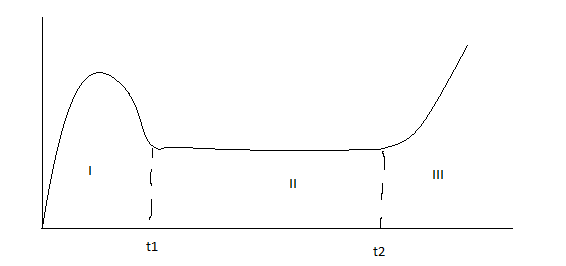
\includegraphics[width=0.6\textwidth]{38_Zhizn2.png}
\caption{Зависимость интенсивности отказов ЭС от времени: I --- 0-t1 период приработки изделия, II --- t1-t2 период эксплуатации изделия, III --- t2-$\infty$ период старения и износа изделия}
\label{fig:Zhizn}
\end{figure}

В 1 периоде отказы ЭРЭ, узлов  происходят из-за: некачественного монтажа, сборки, низкой надежности элементов, контактов, проводников.
Во 2 периоде число отказов стабилизируется , но оно не равно нулю.
В 3 периоде отказы изделия происходят из-за физического старения материалов и износа ЭРЭ, имеющие необратимый характер.
Для нахождения р(t) = F[$\lambda$(t)] проинтегрируем $\lambda(t)$,
\begin{equation}
\int_0^t \lambda (t) =- \int_0^t \frac{dp(t)}{dt} \cdot \frac{1}{p(t)} ,
\end{equation}
\begin{equation}
-\int_0^t \lambda (t)dt = \int_0^t \frac{dp(t)}{p(t)}, -\int_0^t \lambda (t)dt = \ln p(t) ,
\end{equation}
\begin{equation}
p(t) = e^{- \int_{0}^{t} \lambda(t)dt}
\end{equation}

Вероятность безотказной работы имеет экспоненциальный вид, аналогично может быть найдена условная вероятность безотказной работы за интервал времени (t1,t2)
\item \underline{Средняя наработка до отказа}
Tcp(t) --- время работы изделия до первого отказа.
\begin{equation}
T_{cp} (t)= \int_0^\infty p(t)dt,
\end{equation}
Статистически оно находится
\begin{equation}
T^{*}_{cp} (t) = \frac{1}{N_0} \sum_{i=1}^{N_0} t_i,
\end{equation}
где $t_i$ --- время работы до отказа i-го однотипного изделия.
Рассмотрим расчет показателей надежности ЭС для 2 периода $ \lambda(t)=const = \lambda$
\begin{equation}
p(t)= e^{- \lambda t},
\end{equation}
\begin{equation}
T_{cp}(t) = \int_0^\infty p(t)dt= \int_0^\infty e^{- \lambda t}dt = \frac{1}{\lambda},
\end{equation}
Рассмотренные показатели надежности справедливы для невосстанавливаемых ЭС.
\end{enumerate}

\section{Последовательная модель надежности ЭС.}
%Вопрос №39

При последовательном соединении элементов расчет надежности производят по формуле %formula

\begin{equation}
P_A(t) = {\prod_{i=1}^{m}p_i(t) }
\end{equation}
Для большего значения вероятности безотказной работы каждый элемент должен иметь значение вероятности безотказной работы близкой к единице.\\
$P_A(t)\leqslant1$,
 при увеличении количества компонентов в ЭС надежность его падает.(пример)
В тех случаях , когда нужна высокая надежность ЭС, а элементы имеют небольшое значения вероятности безотказной работы, применяют метод резервирования.

Пример:
\begin{figure}[H]
\centering
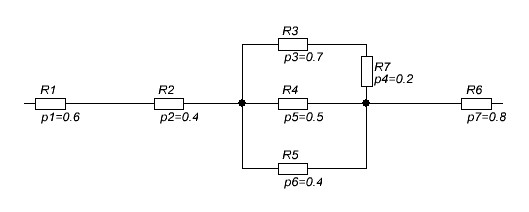
\includegraphics[width=0.8\textwidth]{39_primer.JPG}
\caption{цепь резисторов}
\end{figure}
найти вероятность безотказной работы цепи резисторов.\\
Решение: $P_A = p_1 \cdot p_2 \cdot p_7 \cdot (1-(1-p_3\cdot p_4)(1-p_5)(1-p_6)) $ подставим значения и получим $P_A = 0.6 * 0.4 * 0.8 * (1-(1-0.7*0.2)(1-0.5)(1-0.4))=0.6 * 0.4 *0.8 * (1-0.86*0.5*0.6)= 0.6*0.4*0.8*0.742 = 0.142464$

\section{Параллельная модель надежности ЭС.}
%Вопрос №40

При параллельном соединении элементов расчет надежности производят по формуле 
\begin{equation}
P_A(t) = {1- \prod_{i=1}^{m}[1-p_i(t)] }
\end{equation}
\begin{figure}[H]
\centering
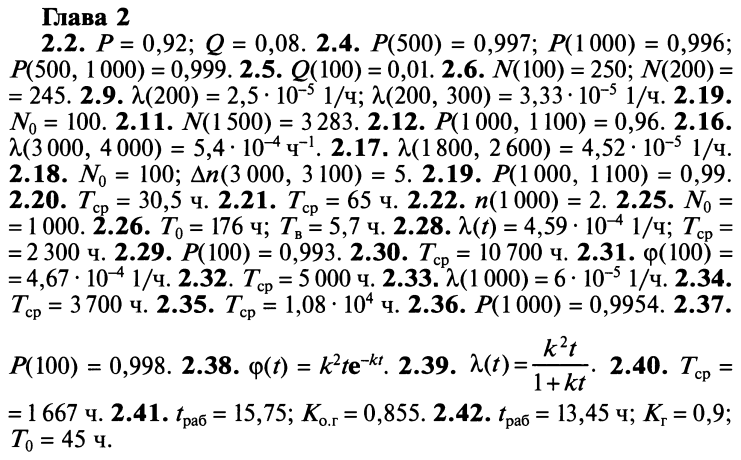
\includegraphics[width=0.8\textwidth]{40_Otvet2.png}
\caption{Ответы ))}
\end{figure}
\begin{figure}[H]
\centering
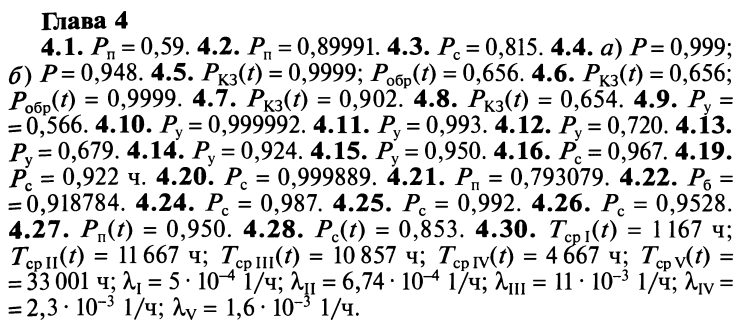
\includegraphics[width=0.8\textwidth]{40_Otvet4.png}
\caption{Ещё ответы}
\end{figure}

\end{document}